\documentclass[12pt,letterpaper,boxed]{hmcpset}
\usepackage{float}
\restylefloat{figure}
\usepackage{graphicx}
\usepackage{amsmath}


\name{Lujia Zhang}
\class{CSSE 477}
\mailbox{CM 1405}
\assignment{Paper Review 3}

\begin{document}

\begin{problem}[1. What are the three essential components of the World Wide Web (WWW) or in short, the web?]
\end{problem}
A demand content, client and servers.


\begin{problem}[2. What is the key advantage of having layered architecture for the Internet when it comes to building applications
using HTTP?]
\end{problem}
HTTP doesn’t need to worry about data loss since it will be handled within the transport layer (TCP) during connection.


\begin{problem}[3. HTTP is a stateless protocol. Explain why?]
\end{problem}
Each HTTP request to a server is considered a brand new one, so aside from the aide of cookies, the server doesn’t connect individual requests. Therefore it retains no information about the users or clients . So it's stateless.

\begin{problem}[4. Assume you have entered the following URL on your browser: http://everest.csse.rose-hulman.edu/index.html.
(Please check the contents of the web page before you answer this question.) Assume the browser uses non- persistent connection to the server. List down the sequence of activities that happens before the browser displays the content of the page.]
\end{problem}
\begin{itemize}
	\item a. HTTP client opens a TCP connection with http://everest.csse.rose-hulman.edu on port 80. 
    \item b. HTTP client sends a request over the TCP connection for index.html
    \item c. http://everest.csse.rose-hulman.edu processes the request, packages it in an HTTP response and sends it back to the client
    \item d. http://everest.csse.rose-hulman.edu tells the TCP connection to close when the client has received the message
    \item e. HTTP client receives the response, closes the TCP connection, and displays the text.
    \item f. steps 4a-d are repeated for the image
    \item g. after the client receives the image, it closes the TCP connection and displays it.
\end{itemize}


\begin{problem}[5. What is the difference if the browser uses persistent connection for question \#4?]
\end{problem}
Because the connection would persist and not be closed the three-way handshake wouldn’t need to happen between each connection. The TCP connection would not be broken and could be used to transfer each file.


\begin{problem}[6. What is the key advantage of having persistent connection?]
\end{problem}
Since multiple objects can be sent over the same TCP connection, entire web pages can be sent over the same connection, which reduces loading times. There is no need to open a new connection for the transfer of each file.


\begin{problem}[7. Give a short description for each of the following field (or line) in an HTTP request message:\newline
a. GET $/~test/index.html$ HTTP/1.1 \newline
b. Host: everest.csse.rose-hulman.edu]
\end{problem}
\begin{itemize}
\item a. GET refers to the type of request. In this case, GET means the 	server should respond with an object. /~test/index.html is the 			object the request wants. HTTP/1.1 is the version of the request.
\item b. Host: serg.csse.rose-hulman.edu is a header that specifies where to direct the request.
\end{itemize}


\begin{problem}[8. Explain the purpose of the following request types: GET, POST, PUT, DELETE, and HEAD.]
\end{problem}
\begin{itemize}
\item a. GET – to retrieve something from the server
\item b. POST – used when a user fills out a form
\item c. PUT – to add something to the server
\item d. DELETE – to remove something from the server
\item e. HEAD – used for debugging

\end{itemize}

\begin{problem}[9. Give a short description of each of the following HTTP response codes: 200, 301, 400, 404, and 505.]
\end{problem}
\begin{itemize}
\item a. 200 – Nothing failed; request received/ processed and info in the response
\item b. 301 – Requested file has been permanently moved to the location in the Locatoin: header.
\item c. 400 – Generic error for bad request.
\item d. 404 – File not found
\item e. 505 – HTTP version not supported by the server


\end{itemize}


\begin{problem}[10. What technique can one use to achieve a stateful behavior while using HTTP?]
\end{problem}
Use cookies.

\begin{problem}[11. How does web caching works?]
\end{problem}
The web cache locally stores files. When the browser establishes a connection to the web cahce it sends an http request
to that cache. The chace checks to see if it has it, if it does it returns the response message which was cached. If not it sends a request for the object to the server, and the server sends a response back to cache. Cache then stores it’s copy and sends it back to the client.

\begin{problem}[12. What is the significance of the conditional-GET request? How do you think the modern-day browsers take
advantage of the conditional-GET requests?]
\end{problem}
The conditional get basically sends a request with a time, which says only send the object back if it has been modified since then. Because the server doesn’t have to send the whole object back if it hasn’t been modified, this is faster and uses less bandwidth. A browser could take advantage of this by locally caching items on the back button. This will make previously viewed websites faster and make hitting the back button faster.

\begin{problem}[13. Download the HTTPTestClient.jar software from Moodle (or use Postman or Advanced REST Client browser
extensions for this exercise). Double-click to run it (or in terminal, type: java –jar HTTPTestClient.jar). Click Connect -> Generate Persistent Request -> Send. You should get a response back. (Note: The connection closed dialog is expected. You should see the response header in the log to understand why. Please feel free to try out other commands too.) \newline
a. Break-down the request according to Figure 2.8. (i.e., Identify request line, header lines, blank line, and entity body). \newline
b. Break-down the response according to Figure 2.9.]
\end{problem}
 \begin{figure}[H]
  \centering
  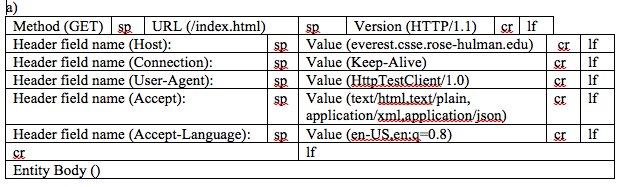
\includegraphics[width = 1.0\textwidth]{1.png}
\end{figure}

 \begin{figure}[H]
  \centering
  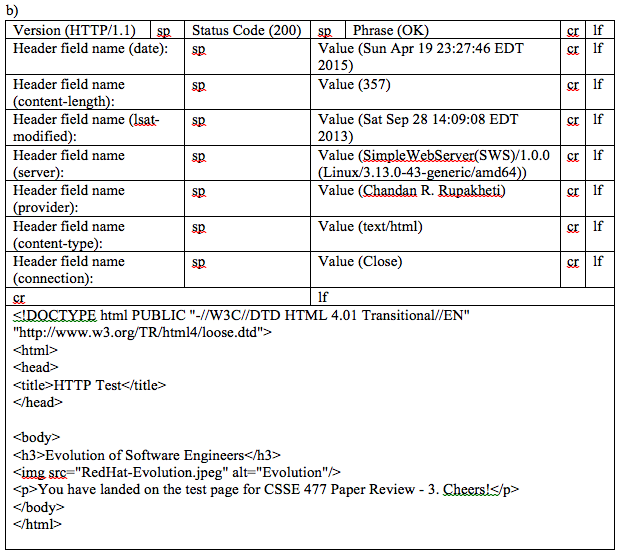
\includegraphics[width = 1.0\textwidth]{2.png}
\end{figure}

\begin{problem}[14. Based on your new found understanding of HTTP and Web Servers, if you were tasked with developing a Web
Server from scratch in either Java or C\#, explain what API you would use for communication between Web Browsers and Web Server? Draw an architecture diagram for the Web Server (not the client) identifying various modules required for the server. Detail the architecture using UML class diagrams where you identify various interfaces and classes in each module. Please briefly describe the purpose of each class and module if it is not very clear just from its name. The latest version of UMLet can be downloaded from Moodle (under the Resources section) that you can use for drawing. (Note that I am looking for a meaningful attempt here, which does not have to be absolutely correct.)]
\end{problem}
If implemented in Java, I would use various classes in com.sun.net.httpserver such as HttpServer and HttpHandler to build a basic web server.\newline
The following would be my basic implementation using the api \newline com.sun.net.httpserver: \newline
 \begin{figure}[H]
  \centering
  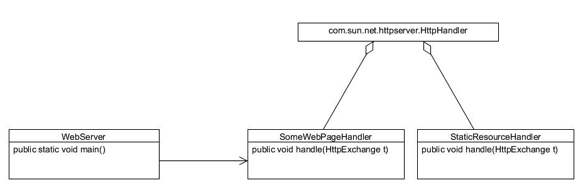
\includegraphics[width = 1.0\textwidth]{3.png}
\end{figure}
WebServer is the main that controls all mappings for pages such as index.html and \newline IndexPageHandler and any static resources (.CSS or .JS) and StaticResourceHandler. \newline IndexPageHandler would then be in charge of knowing the location of index.html and how to respond to the request. 




\end{document}